\documentclass[10pt,letterpaper]{article}

\usepackage[utf8]{inputenc}
\usepackage[T1]{fontenc}
\usepackage{booktabs}
\usepackage{graphicx}
\usepackage{tabularx}
\usepackage{array}
\usepackage{makecell}
\usepackage{enumitem}
\usepackage{geometry}
\usepackage{microtype}
\usepackage{parskip}
\usepackage{xcolor}
\usepackage{caption}
\usepackage{fancyhdr}
\usepackage{hyperref}

\geometry{letterpaper,margin=0.68in}
\setlength{\emergencystretch}{3em}
\setlength{\parskip}{4pt}
\setlength{\parindent}{0pt}
\setlist{leftmargin=*,itemsep=2pt,topsep=3pt,parsep=0pt}
\captionsetup{font=small,labelfont=bf}

\definecolor{cmured}{HTML}{C41230}
\definecolor{muted}{HTML}{666666}
\hypersetup{
  colorlinks=true,
  linkcolor=cmured,
  urlcolor=cmured,
  pdftitle={Efficient Coverage Playbook: Comparing Predictive Uncertainty Across Model Classes for NFL Big Data Bowl Problems},
  pdfauthor={Jonathan Pipping-Gamon and Ron Yurko}
}

\pagestyle{fancy}
\fancyhf{}
\fancyhead[L]{\small\textcolor{muted}{Efficient Coverage Playbook}}
\fancyhead[R]{\scriptsize\textcolor{muted}{Comparing Predictive Uncertainty Across Model Classes for NFL Big Data Bowl Problems}}
\fancyfoot[C]{\thepage}
\renewcommand{\headrulewidth}{0.25pt}

\newcolumntype{Y}{>{\raggedright\arraybackslash}X}
\newcolumntype{C}{>{\centering\arraybackslash}X}
\newcolumntype{P}[1]{>{\raggedright\arraybackslash}p{#1}}
\newcommand{\role}[1]{\textbf{#1}}
\newcommand{\clearwinner}[1]{\textbf{#1}\textsuperscript{*}}
\newcommand{\sourcepath}[1]{\texttt{\detokenize{#1}}}

\begin{document}

\begin{center}
  {\LARGE\bfseries Efficient Coverage Playbook\par}
  \vspace{0.35em}
  {\large\textcolor{cmured}{Comparing Predictive Uncertainty Across Model Classes for NFL Big Data Bowl Problems}\par}
  \vspace{0.65em}
  {Jonathan Pipping-Gam\'on \qquad Ron Yurko\par}
  \vspace{0.25em}
  {\small September 2026\par}
\end{center}

\vspace{0.4em}
\hrule
\vspace{0.75em}

This packet summarizes the completed BDB2020--2025 analyses. Each problem uses 100 complete game-level repetitions and a sequence of nested training-game budgets. The same games are assigned to every model within a repetition. BDB2026 is not included in the completed evidence summarized here.

\section*{Results at a glance}

\begin{itemize}
  \item \role{Rushing yards:} the Set Transformer is the clear CRPS winner at all six training-game budgets. At valid empirical coverage, LightGBM gives the narrowest intervals at the largest budget.
  \item \role{Pass completion and tackle candidates:} the clearest primary-loss results favor structured tabular models. Completion shifts from regularized regression at small budgets to boosted trees at 100 and 130 games. Boosted trees are clear at every tackle budget.
  \item \role{Punt returns and sacks:} the observed rankings remain close enough that no model is a clear winner under the problem-wide max-$t$ rule.
  \item \role{Man/Zone:} boosted trees are clear at 20--40 games. At 60 games, the Set Transformer has the lowest observed mean Brier score, but the simultaneous comparison does not identify a clear winner.
\end{itemize}

\section*{Six completed football problems}

\footnotesize
\setlength{\tabcolsep}{4pt}
\begin{tabularx}{\textwidth}{@{}lYlllY@{}}
\toprule
Problem & Question & Prediction moment & Output & Primary loss & Training-game budgets \\
\midrule
BDB2020 & Rushing yards & Handoff & Yard distribution & CRPS & 20, 40, 80, 160, 240, 360 \\
BDB2021 & Pass completion & Pass release & Probability & Brier & 10, 20, 40, 60, 100, 130 \\
BDB2022 & Punt-return yards & Punt received & Yard distribution & CRPS & 10, 20, 40, 60, 160, 360 \\
BDB2023 & Sack & Snap & Probability & Brier & 10, 20, 30, 40, 50, 60 \\
BDB2024 & Tackle candidate & Candidate event minus 10 frames & Candidate probability & Brier & 10, 20, 30, 40, 50, 60 \\
BDB2025 & Man/Zone & Final 20 frames through snap & Probability & Brier & 10, 20, 30, 40, 50, 60 \\
\bottomrule
\end{tabularx}
\normalsize

\clearpage
\section{Common experimental design}

The independent resampling unit is the \textbf{game}. Within each repetition, every model receives the same training, calibration, and test games and the same nested order of training games. The 100 repetitions therefore provide paired procedural comparisons while allowing the sampled games and neural initialization to vary.

\subsection*{Model roles}

The recurring BDB2021--2025 panel separates the information representation from the fitting algorithm. BDB2020 uses an earlier four-model panel.

\small
\begin{tabularx}{\textwidth}{@{}P{3.1cm}P{4.3cm}Y@{}}
\toprule
Model role & Input & Estimator \\
\midrule
Linear-Structure & Engineered football features & Regularized linear or logistic model \\
Boosted-Structure & The same engineered features & Gradient-boosted decision trees \\
RelNet & Player-by-frame tracking and typed football graph & One shared pairwise MLP with pooled messages \\
AttnRelNet & The same tracking sequence and graph & The same messages with learned attention weights \\
Global Set Transformer & Player-by-frame tracking without a specified graph & Player attention followed by temporal attention \\
\bottomrule
\end{tabularx}
\normalsize

Stable player identifiers align slots across frames but do not enter the models. Primary models exclude player and team identity. RelNet and AttnRelNet share inputs, edges, temporal encoding, prediction heads, losses, tuning grids, seeds, and training procedures; attention is the intended difference.

\subsection*{Three dimensions of predictive performance}

\begin{itemize}
  \item \role{Accuracy} uses CRPS for a predicted yard distribution and Brier score for a predicted probability. Lower is better.
  \item \role{Uncertainty} asks whether intervals or prediction sets attain their target coverage and how informative they are after coverage is established. Yard problems report interval width. Binary problems report class-conditional conformal-set coverage and singleton rate. Venn--Abers probability ranges are calibration diagnostics, not prediction intervals.
  \item \role{Stability} describes variation across the 100 complete repetitions. Learning-curve bands are the 10th and 90th percentiles across repetitions.
\end{itemize}

For formal model comparisons, each problem uses paired loss differences and a 95\% max-$t$ bootstrap over the full comparison family. BDB2021--2025 contain ten model pairs at six budgets, or 60 simultaneous comparisons per problem. The earlier BDB2020 analysis protects a broader 324-comparison family that includes 36 CRPS contrasts. A \emph{clear winner} must beat every alternative at the same budget under the relevant simultaneous intervals. The max-$t$ bootstrap resamples complete repetition vectors, preserving dependence induced by shared models, games, and budgets. The descriptive 10th--90th percentile ribbons do not determine the clear-winner label.

\clearpage
\section{Model rankings across problems}

\begin{figure}[ht]
\centering
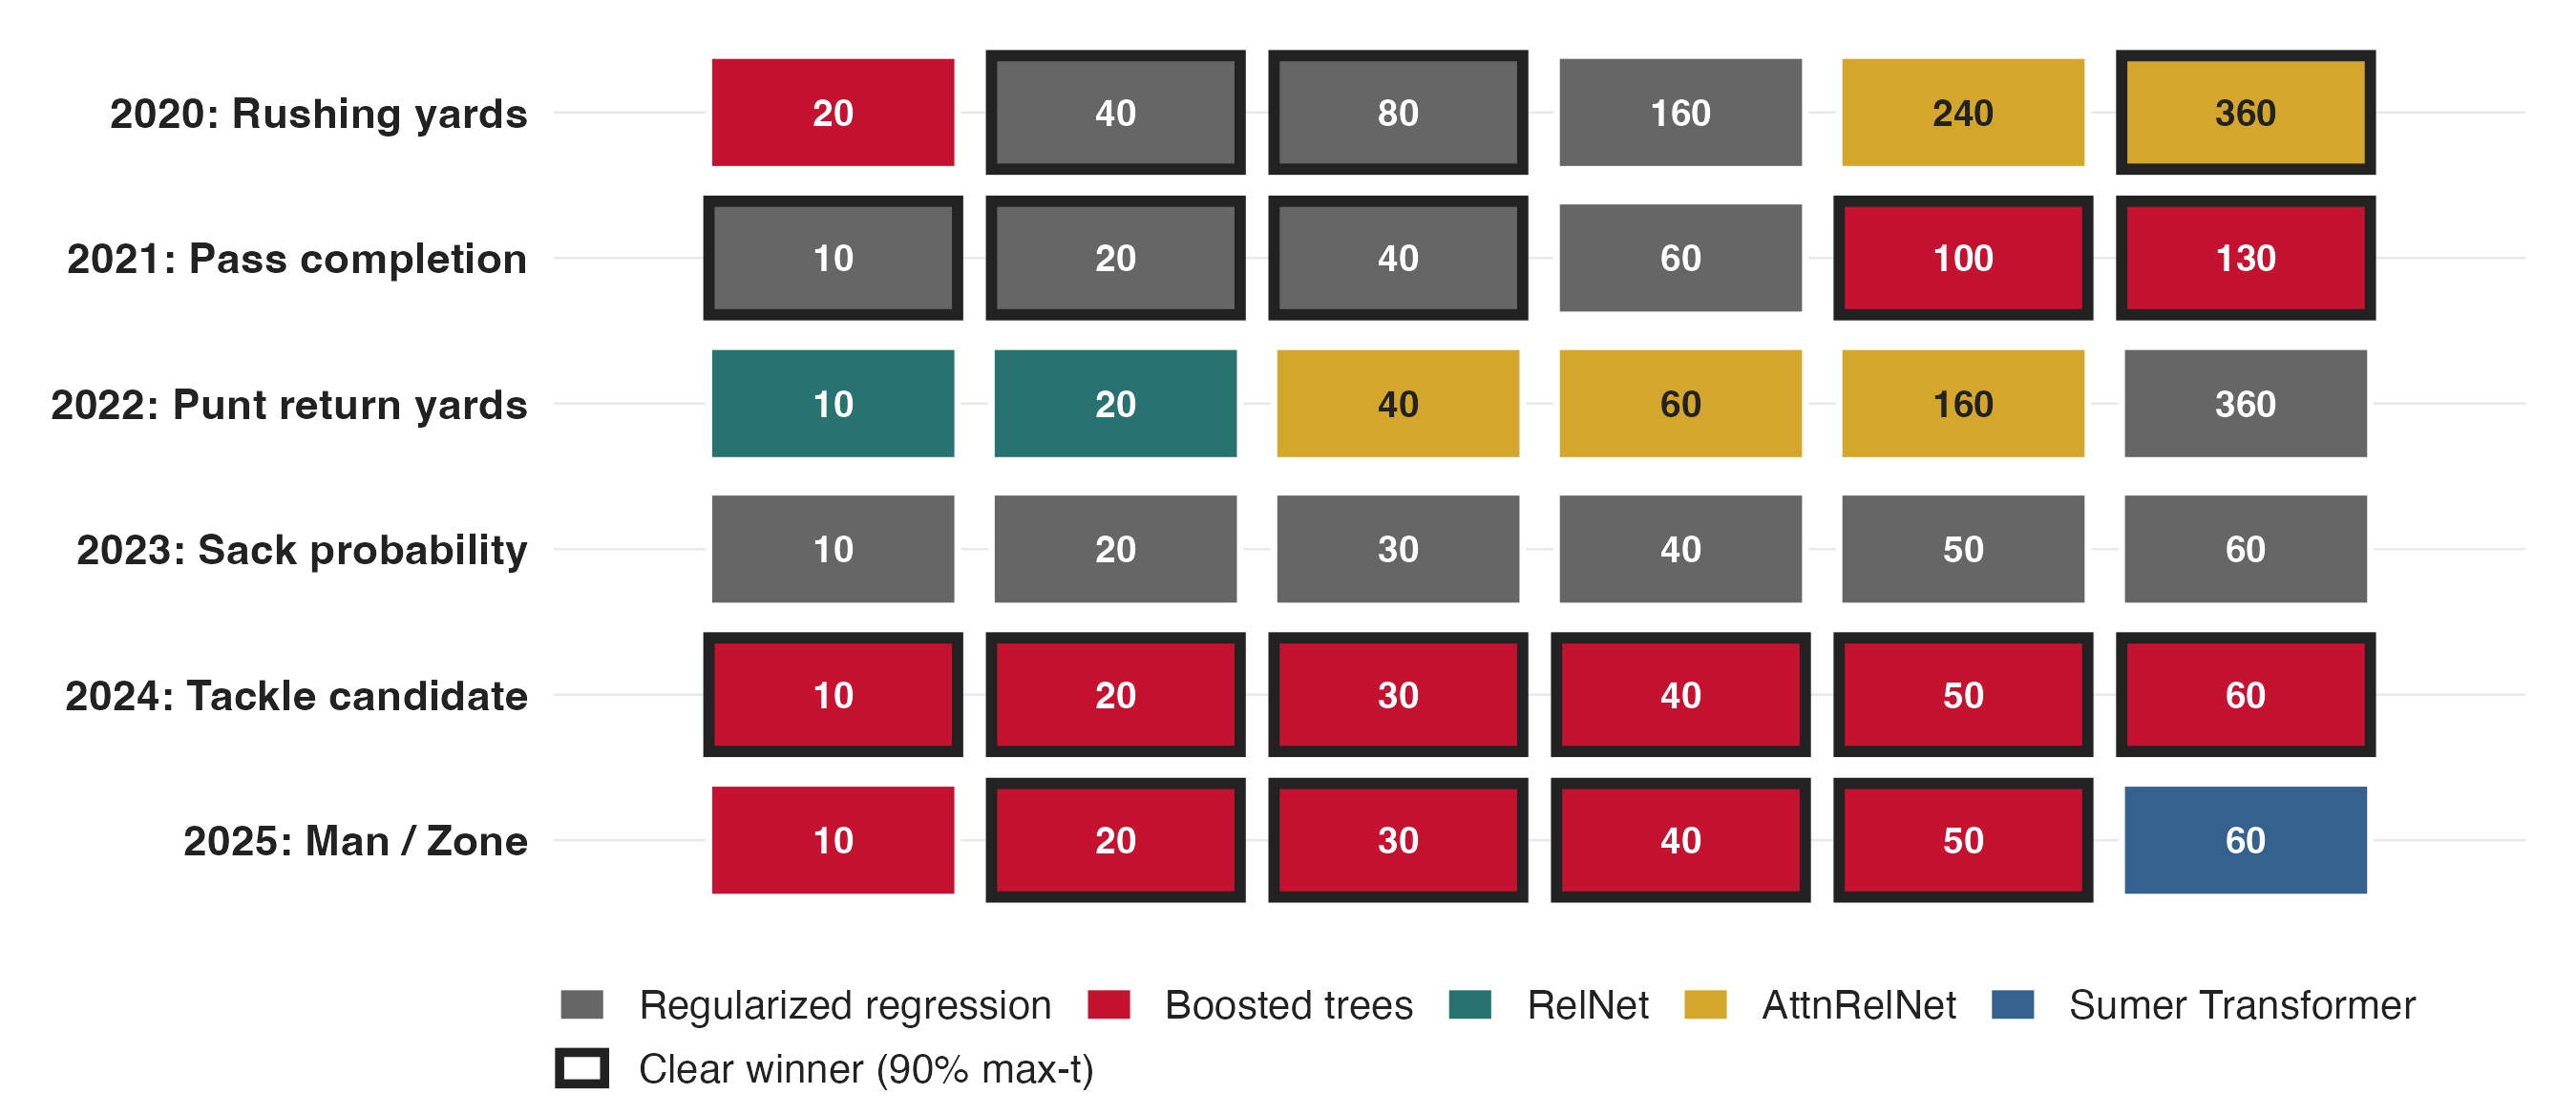
\includegraphics[width=0.98\textwidth]{../presentations/cassis2026/figures/supported_winner_matrix.png}
\caption{Lowest observed mean primary loss by task and training-game budget for BDB2021--2025. Dark outlines mark budgets where problem-wide 95\% max-$t$ comparisons identify that model as the clear winner.}
\end{figure}

Across BDB2021--2025, 14 of 30 task-budget cells identify a clear winner. Boosted-Structure accounts for 11 and Linear-Structure for three. The neural classes have the lowest observed mean in six cells but are not clear winners in this five-problem family. BDB2020 is the important separate case: the Set Transformer is the clear CRPS winner at all six budgets in its four-model panel. None of the 30 matched RelNet--AttnRelNet primary-loss comparisons identifies a clear difference; this does not establish equivalence.

\clearpage
\section{Performance at the largest game budget}

Table~\ref{tab:largest-primary} reports the mean primary loss and its SD across 100 repetitions for the common five-model panel. Each column is comparable within a problem only. Bold entries have the lowest observed mean. An asterisk marks a clear winner under the 95\% problem-wide max-$t$ rule.

\begin{table}[ht]
\centering
\caption{Primary loss at the largest training-game budget, mean (SD) across 100 repetitions.}
\label{tab:largest-primary}
\scriptsize
\setlength{\tabcolsep}{3.5pt}
\resizebox{\textwidth}{!}{%
\begin{tabular}{@{}lccccc@{}}
\toprule
Model & \makecell{BDB2021\\Brier, 130 games} & \makecell{BDB2022\\CRPS, 360 games} & \makecell{BDB2023\\Brier, 60 games} & \makecell{BDB2024\\Brier, 60 games} & \makecell{BDB2025\\Brier, 60 games} \\
\midrule
Linear-Structure  & 0.21024 (0.00271) & \textbf{0.03464 (0.00223)} & \textbf{0.06126 (0.00492)} & 0.08642 (0.00582) & 0.13232 (0.00775) \\
Boosted-Structure & \clearwinner{0.20571 (0.00275)} & 0.03634 (0.00220) & 0.06265 (0.00513) & \clearwinner{0.05819 (0.00459)} & 0.11971 (0.00806) \\
RelNet            & 0.21383 (0.00371) & 0.03478 (0.00235) & 0.06137 (0.00488) & 0.05997 (0.00465) & 0.12197 (0.01046) \\
AttnRelNet        & 0.21389 (0.00381) & 0.03480 (0.00237) & 0.06136 (0.00488) & 0.06027 (0.00503) & 0.12162 (0.01072) \\
Set Transformer   & 0.21438 (0.00399) & 0.03523 (0.00244) & 0.06129 (0.00481) & 0.06467 (0.00551) & \textbf{0.11921 (0.00798)} \\
\bottomrule
\end{tabular}}
\end{table}

BDB2020 used a different four-model panel. At 360 games, the Set Transformer has the lowest mean CRPS and remains the clear winner.

\begin{table}[ht]
\centering
\caption{BDB2020 primary loss at 360 training games, mean (SD) across 100 repetitions.}
\small
\begin{tabular}{@{}lcc@{}}
\toprule
Model & Mean CRPS & SD across repetitions \\
\midrule
L2 one-vs-rest logistic & 0.01423 & 0.00025 \\
LightGBM & 0.01334 & 0.00028 \\
Zoo CNN & 0.01295 & 0.00044 \\
Set Transformer & \clearwinner{0.01253} & 0.00026 \\
\bottomrule
\end{tabular}
\end{table}

\clearpage
\section{Uncertainty at the largest game budget}

For yard-distribution problems, width is meaningful only alongside empirical coverage. All entries below exceed the nominal 90\% target at the displayed budget, but the model with the lowest primary loss does not always give the narrowest interval.

\begin{table}[ht]
\centering
\caption{Yard-distribution accuracy and intervals at the largest budget. Means across 100 repetitions.}
\label{tab:yard-uncertainty}
\small
\setlength{\tabcolsep}{5pt}
\begin{tabular}{@{}llrrr@{}}
\toprule
Problem & Model & CRPS & Coverage & Mean width (yards) \\
\midrule
BDB2020, 360 & L2 one-vs-rest logistic & 0.01423 & 93.72\% & 21.59 \\
 & LightGBM & 0.01334 & 91.52\% & \textbf{13.64} \\
 & Zoo CNN & 0.01295 & 91.87\% & 14.11 \\
 & Set Transformer & \textbf{0.01253} & 92.60\% & 14.46 \\
\addlinespace
BDB2022, 360 & Linear-Structure & \textbf{0.03464} & 92.02\% & 31.67 \\
 & Boosted-Structure & 0.03634 & 93.38\% & 35.12 \\
 & RelNet & 0.03478 & 91.80\% & 23.12 \\
 & AttnRelNet & 0.03480 & 91.78\% & 23.16 \\
 & Set Transformer & 0.03523 & 91.67\% & \textbf{22.87} \\
\bottomrule
\end{tabular}
\end{table}

For binary problems, Table~\ref{tab:binary-uncertainty} follows the model with the lowest observed mean raw Brier score at the largest budget. Venn--Abers supplies the calibrated Brier score. Class-conditional conformal sets target 90\% coverage separately for each label; singleton rate measures how often the set makes a one-label call.

\begin{table}[ht]
\centering
\caption{Binary uncertainty summary for the observed lowest-loss model at the largest budget.}
\label{tab:binary-uncertainty}
\scriptsize
\setlength{\tabcolsep}{4pt}
\begin{tabular}{@{}llrrrrr@{}}
\toprule
Problem & Model & Raw Brier & Calibrated Brier & Label 0 coverage & Label 1 coverage & Singleton rate \\
\midrule
BDB2021, 130 & Boosted-Structure & 0.20571 & 0.20627 & 91.00\% & 91.52\% & 34.69\% \\
BDB2023, 60 & Linear-Structure & 0.06126 & 0.06178 & 90.92\% & 90.55\% & 21.99\% \\
BDB2024, 60 & Boosted-Structure & 0.05819 & 0.05867 & 90.29\% & 90.96\% & 89.10\% \\
BDB2025, 60 & Set Transformer & 0.11921 & 0.11689 & 90.70\% & 91.36\% & 65.83\% \\
\bottomrule
\end{tabular}
\end{table}

\clearpage
\section{Full learning curves}

Each curve is the mean across 100 repetitions. Shaded bands are the 10th and 90th percentiles of the complete repeated procedure. They show procedural variation and are not confidence intervals for a pairwise model difference.

\begin{center}
\centering
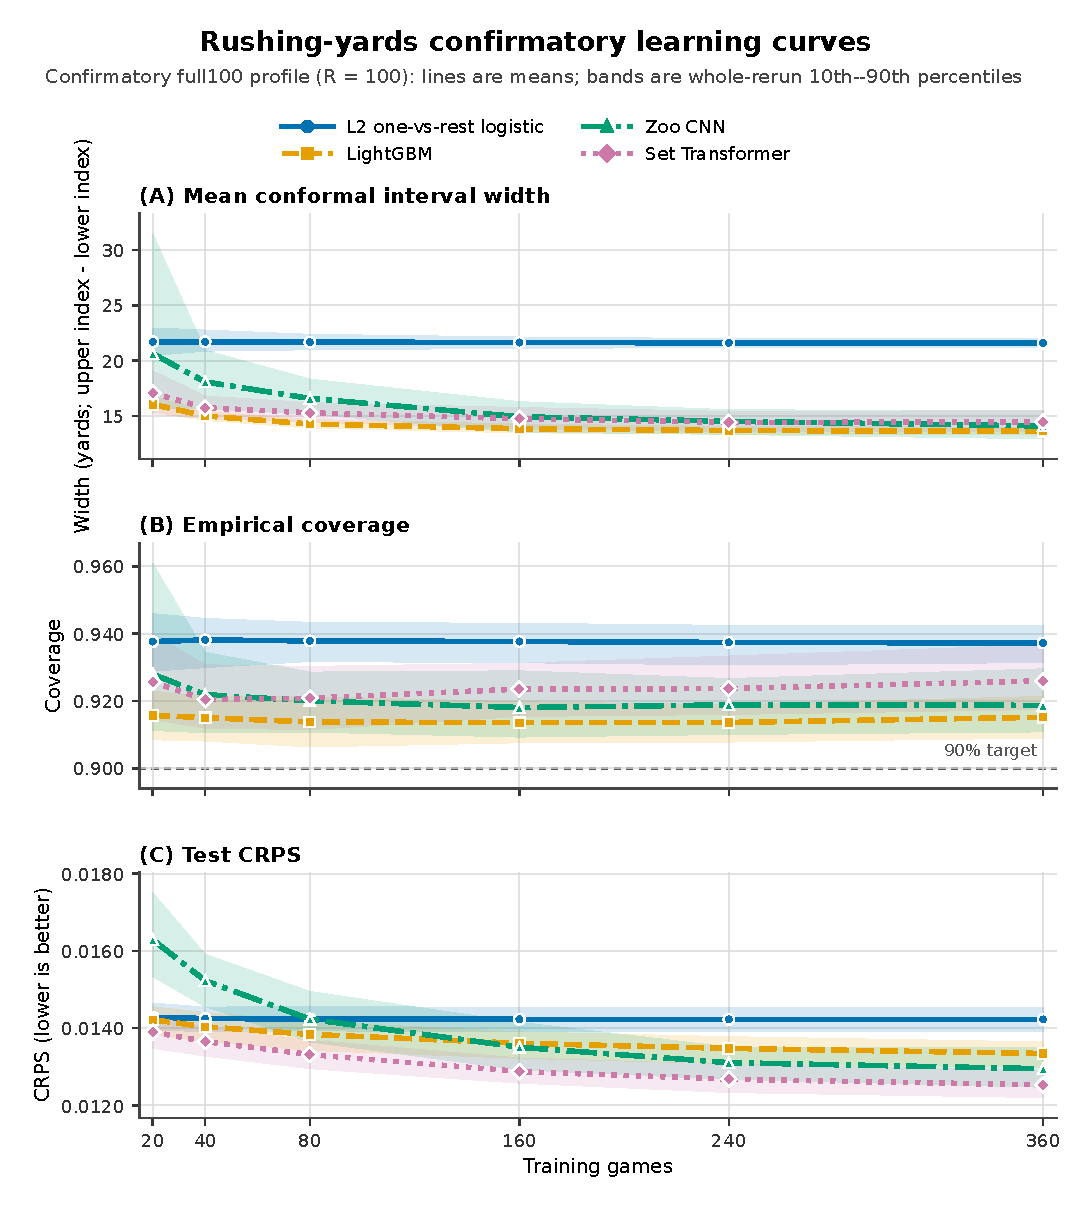
\includegraphics[height=0.73\textheight,width=\textwidth,keepaspectratio]{../results/rushing/full100-confirmatory-20260820/final/main/rushing_confirmatory_100_learning_curves.pdf}
\captionof{figure}{BDB2020 rushing yards.}
\end{center}

\clearpage
\thispagestyle{fancy}
\begin{center}
\centering
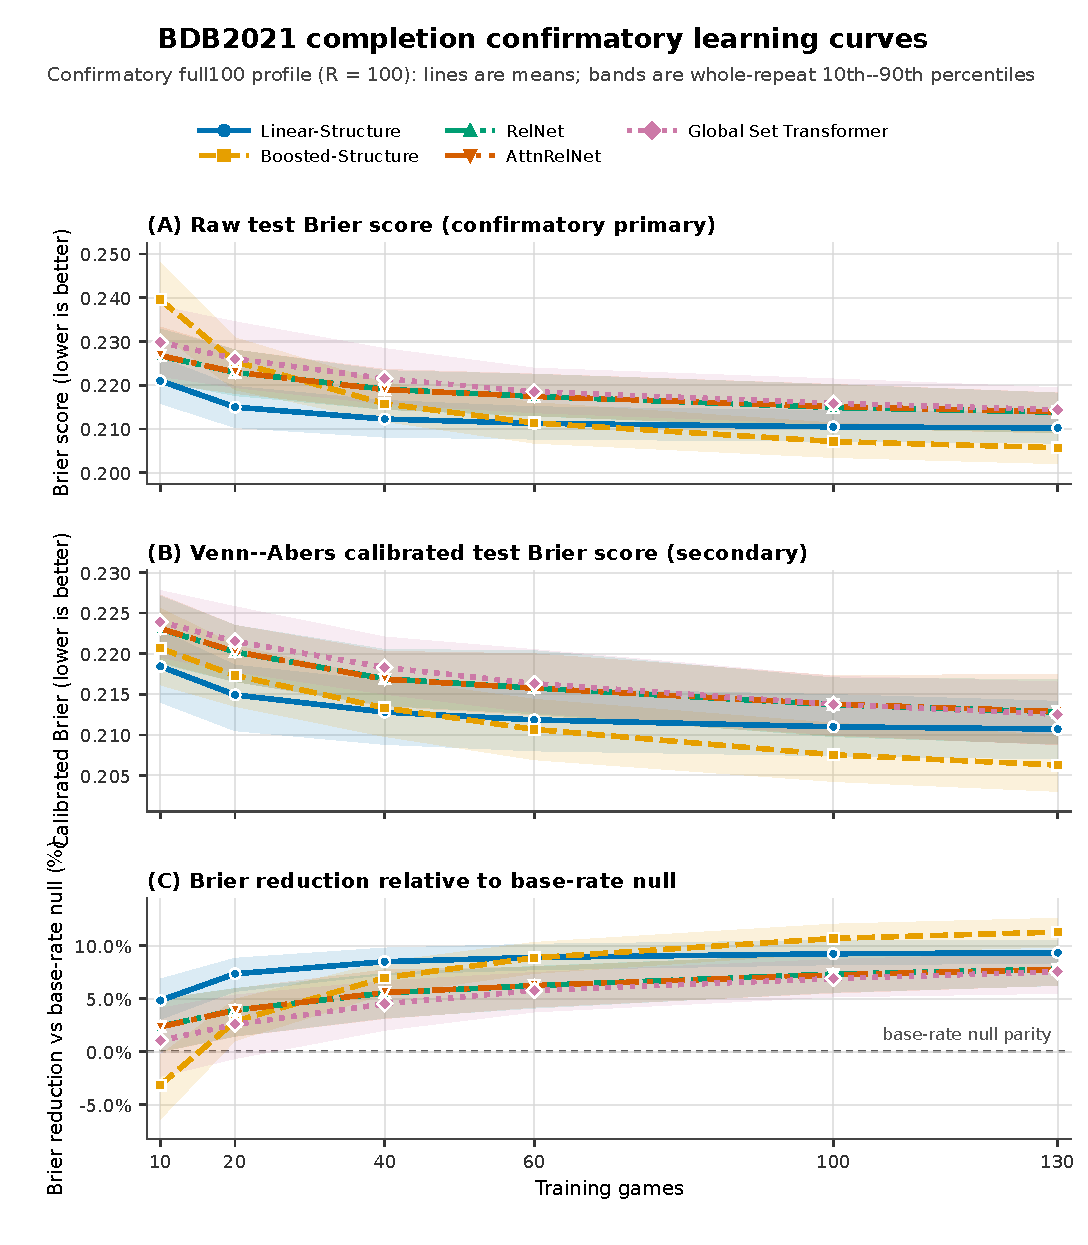
\includegraphics[height=0.86\textheight,width=\textwidth,keepaspectratio]{figures/bdb2021_completion_full100_learning_curves.pdf}
\captionof{figure}{BDB2021 pass completion.}
\end{center}

\clearpage
\thispagestyle{fancy}
\begin{center}
\centering
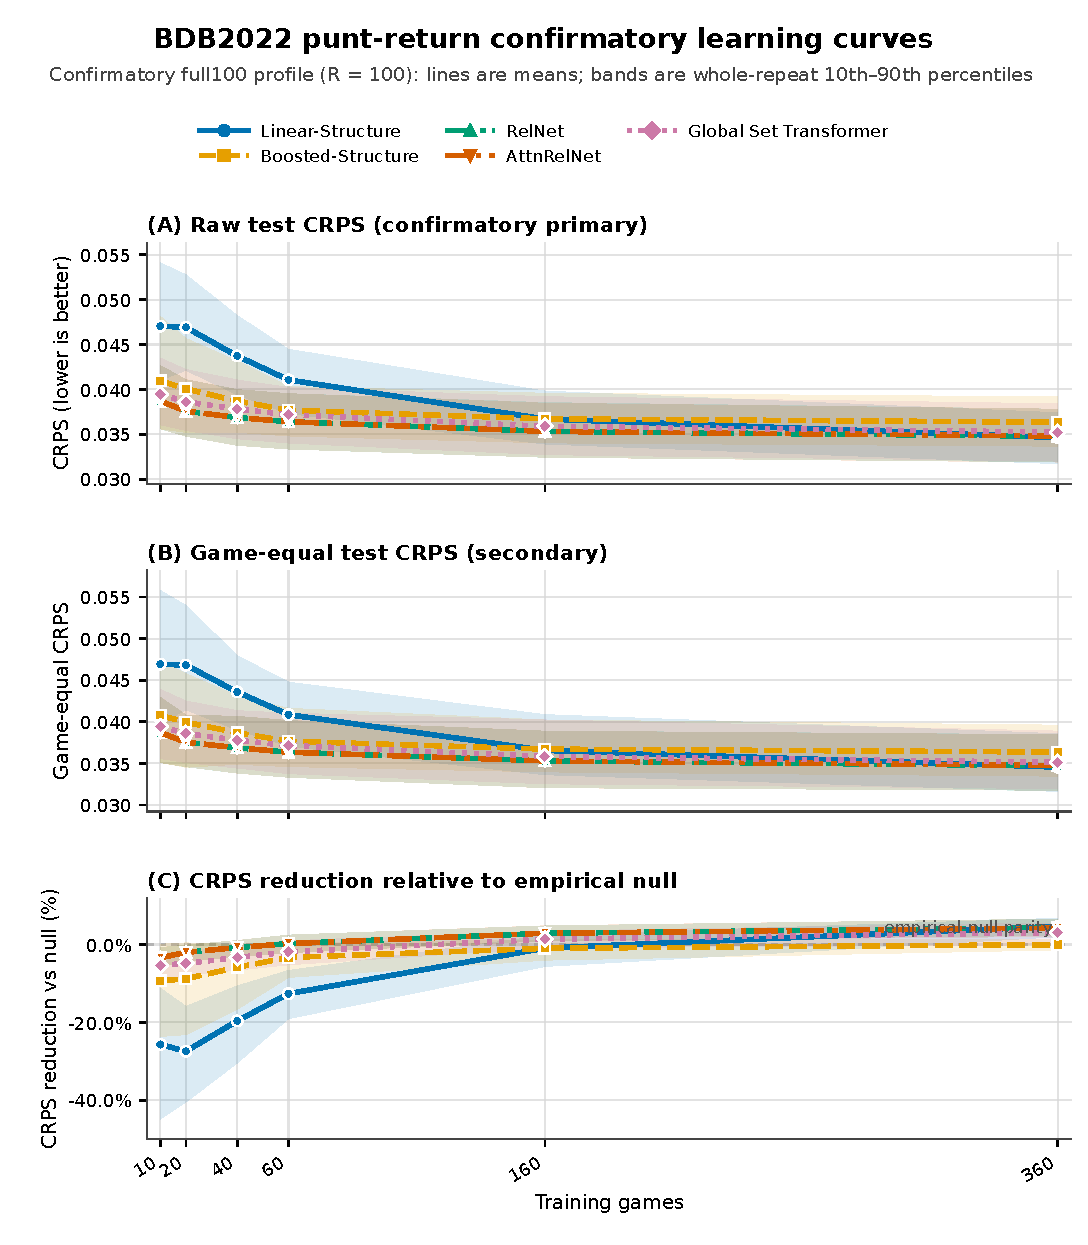
\includegraphics[height=0.86\textheight,width=\textwidth,keepaspectratio]{figures/bdb2022_punt_returns_full100_learning_curves.pdf}
\captionof{figure}{BDB2022 punt-return yards.}
\end{center}

\clearpage
\thispagestyle{fancy}
\begin{center}
\centering
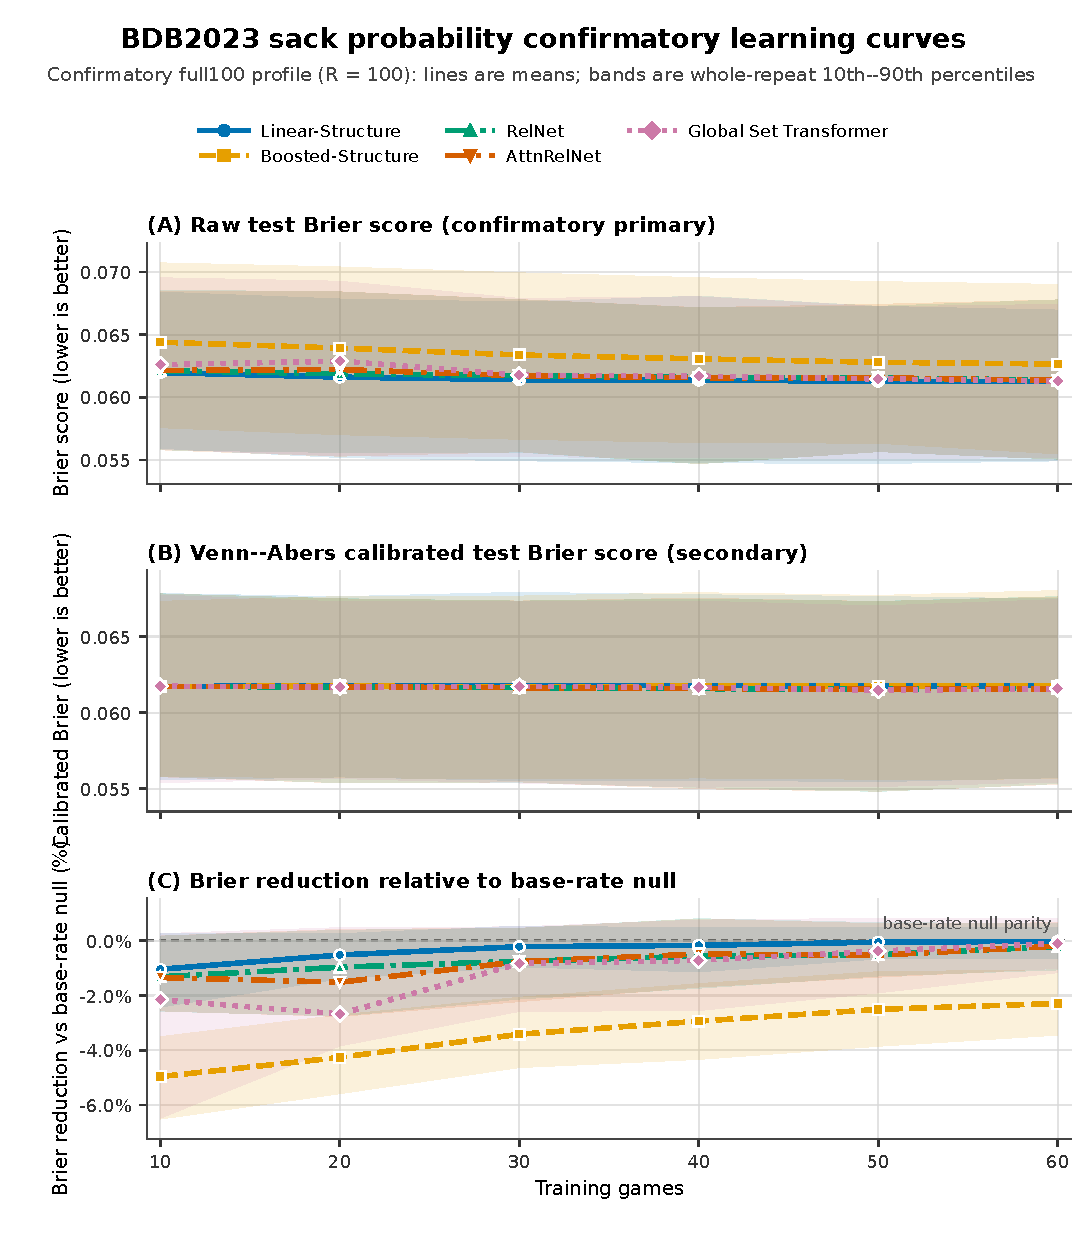
\includegraphics[height=0.86\textheight,width=\textwidth,keepaspectratio]{../results/bdb/full100_serial_bdb2023_attempt1/plots/bdb2023_sack_full100_learning_curves.pdf}
\captionof{figure}{BDB2023 sack probability.}
\end{center}

\clearpage
\thispagestyle{fancy}
\begin{center}
\centering
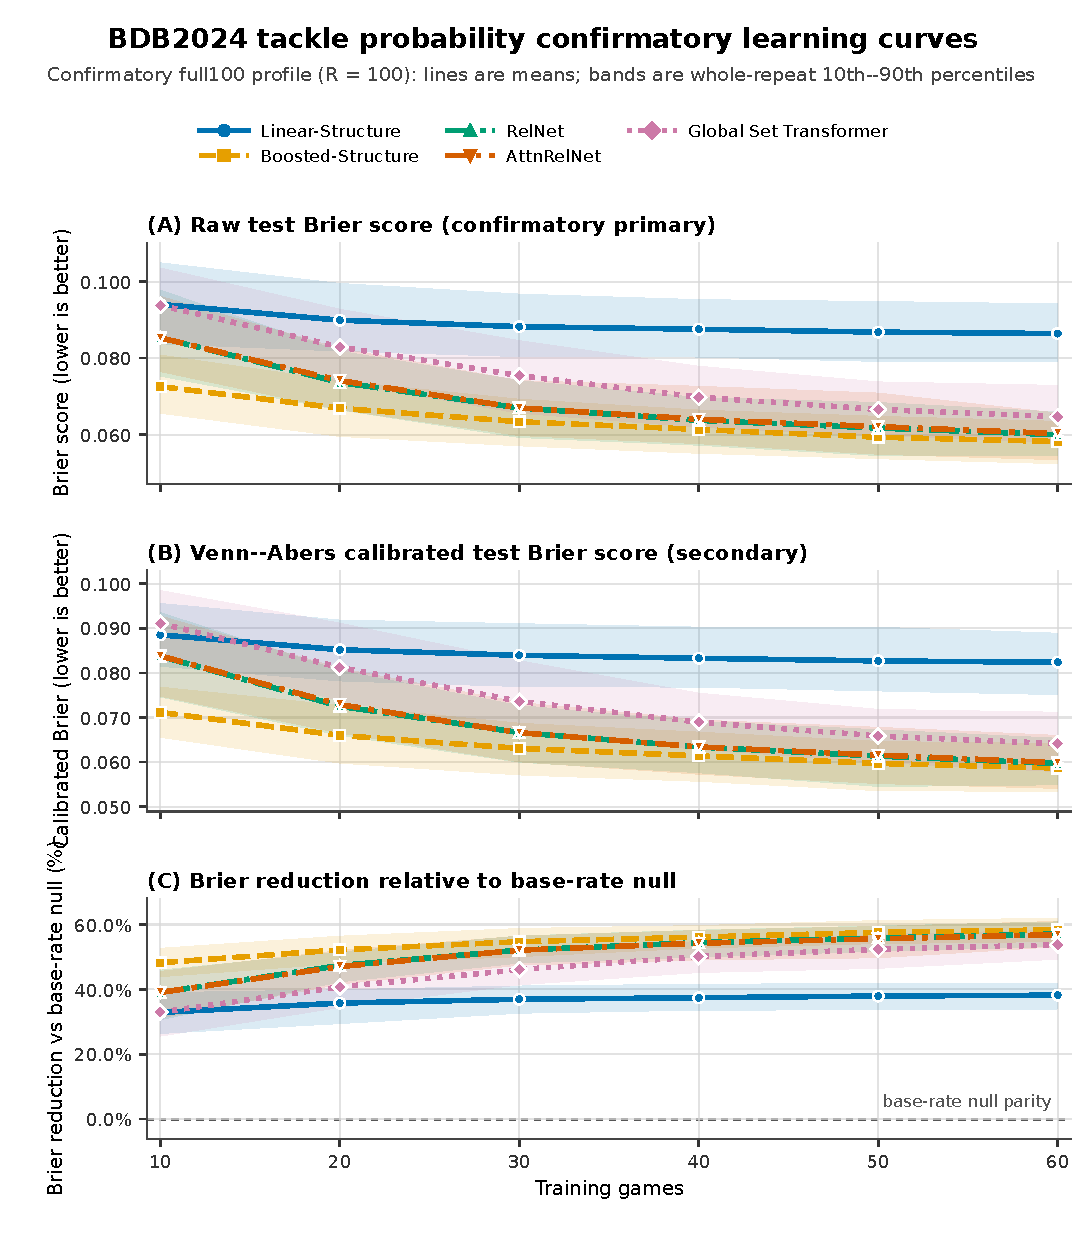
\includegraphics[height=0.84\textheight,width=\textwidth,keepaspectratio]{../results/bdb/full100_serial_bdb2024_attempt1/plots/bdb2024_tackle_full100_learning_curves.pdf}
\captionof{figure}{BDB2024 tackle-candidate probability. This is a candidate-level prediction problem, not an unconditional probability for every defender.}
\end{center}

\clearpage
\thispagestyle{fancy}
\begin{center}
\centering
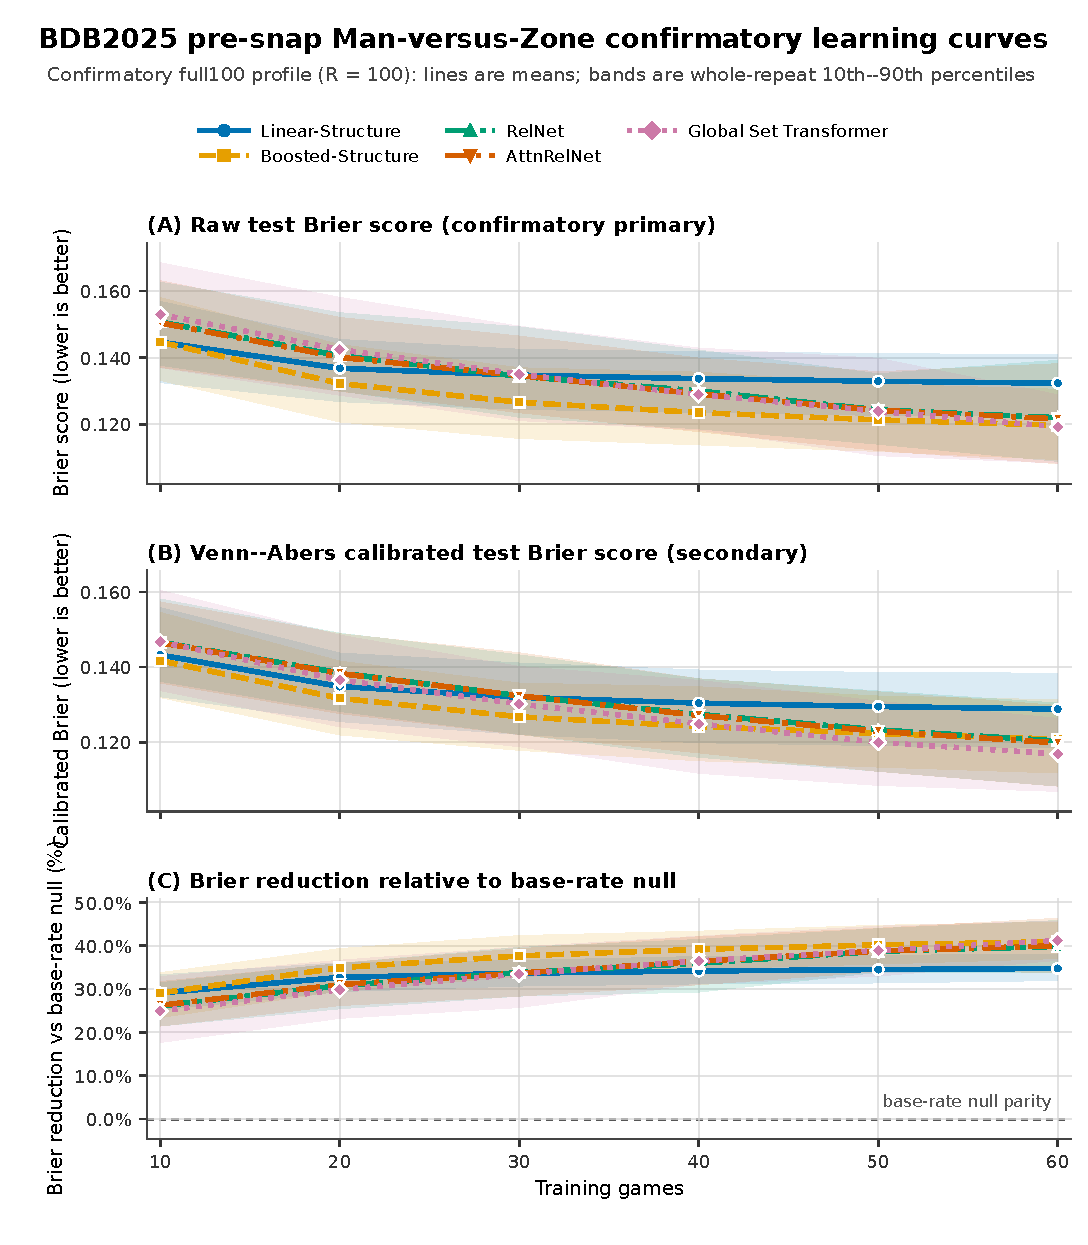
\includegraphics[height=0.86\textheight,width=\textwidth,keepaspectratio]{../results/bdb/full100_serial_bdb2025_attempt1/plots/bdb2025_man_zone_full100_learning_curves.pdf}
\captionof{figure}{BDB2025 pre-snap Man/Zone probability.}
\end{center}

\clearpage
\section{Interpretation and evidence boundary}

The completed problems do not produce a single model ranking. Representation matters, but its value depends on the football question and the available games. Flexible tracking models dominate rushing accuracy, structured tabular models dominate the clearest classification results, and some problems remain unresolved even after 100 repetitions.

\begin{itemize}
  \item A large tracking table does not imply a large independent sample. Repetitions, calibration, and model comparisons operate at the game level.
  \item Point estimates always rank the models. The clear-winner label requires a separate paired max-$t$ comparison across the full prespecified family.
  \item Intervals and sets need to attain their target coverage. Among procedures that do, width or singleton rate distinguishes more informative uncertainty statements.
  \item No clear difference is not evidence of equivalence. This caveat is especially important for the matched RelNet--AttnRelNet comparisons.
\end{itemize}

\subsection*{BDB2026}

BDB2026 requested-player trajectory prediction remains outside this packet's completed empirical evidence. The planned uncertainty object is a whole-path conformal tube: a disk around each predicted point, scaled over forecast horizon, with coverage defined for the complete requested-player path. No BDB2026 number should be combined with the terminal BDB2020--2025 results until its final aggregate and completion receipt are available.

\subsection*{Terminal evidence map}

\scriptsize
\begin{tabularx}{\textwidth}{@{}lY@{}}
\toprule
Problem & Terminal tables and figures \\
\midrule
BDB2020 & \sourcepath{results/rushing/full100-confirmatory-20260820/final/main/} \\
BDB2021 & \sourcepath{presentations/cassis2026/data/raw_terminal/bdb2021/} and \sourcepath{paper/figures/} \\
BDB2022 & \sourcepath{presentations/cassis2026/data/raw_terminal/bdb2022/} and \sourcepath{paper/figures/} \\
BDB2023 & \sourcepath{results/bdb/full100_serial_bdb2023_attempt1/final/} and \sourcepath{results/bdb/full100_serial_bdb2023_attempt1/plots/} \\
BDB2024 & \sourcepath{results/bdb/full100_serial_bdb2024_attempt1/final/} and \sourcepath{results/bdb/full100_serial_bdb2024_attempt1/plots/} \\
BDB2025 & \sourcepath{results/bdb/full100_serial_bdb2025_attempt1/final/} and \sourcepath{results/bdb/full100_serial_bdb2025_attempt1/plots/} \\
\bottomrule
\end{tabularx}
\normalsize

\end{document}
